\documentclass[border=8pt]{standalone}
\usepackage{amsmath}
\usepackage{amssymb}
\usepackage{tikz}
\usetikzlibrary{arrows.meta,calc,decorations.pathreplacing,patterns,shapes.geometric,positioning,shadings,plotmarks}

\begin{document}
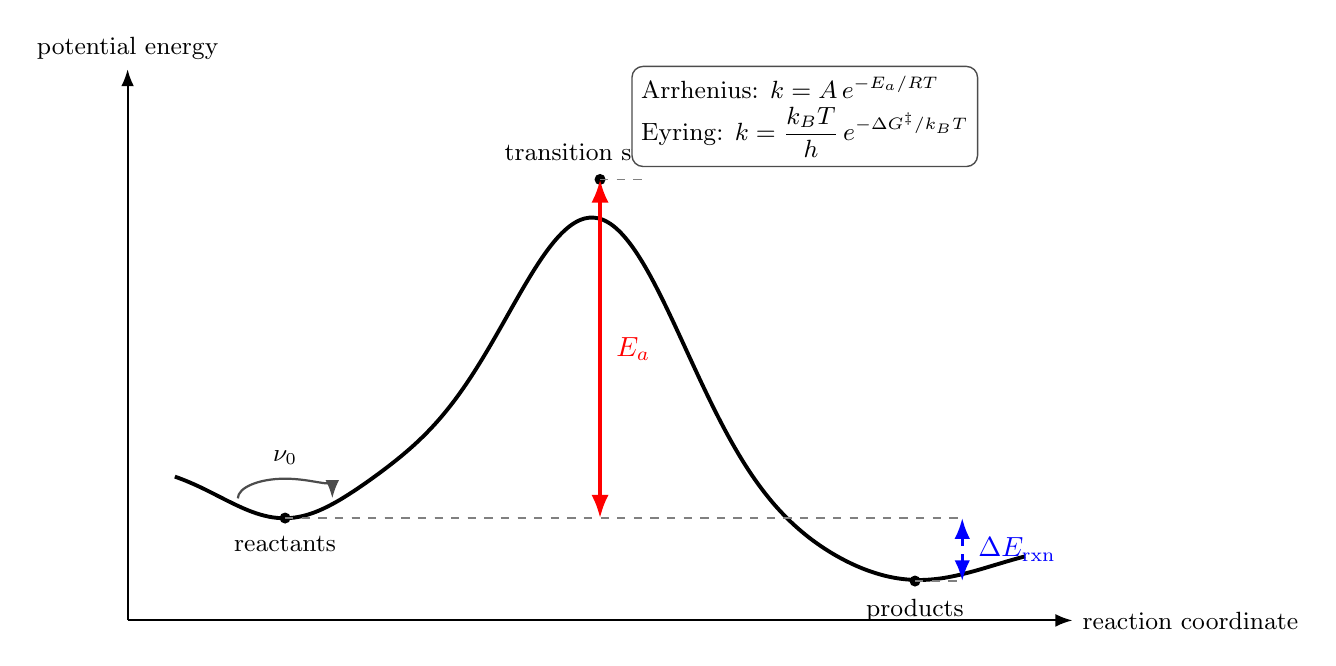
\begin{tikzpicture}[>=Latex,thick]

% Axes
\draw[->, line width=0.7pt] (0,0) -- (12,0) node[right] {\small reaction coordinate};
\draw[->, line width=0.7pt] (0,0) -- (0,7) node[above] {\small potential energy};

% Potential energy curve: reactants well (left, slightly higher) -> peak (TS) -> products well (right, lower)
% reactants well bottom: (2, 2.0)
% TS peak: (6, 5.6)
% products well bottom: (10, 1.0)
\draw[black, line width=1.4pt, smooth, samples=200, domain=0.6:11.4]
  plot (\x, { 2.0 + 3.6*exp(-((\x-6)*(\x-6))/2.5) - 1.0/(1+exp(-(\x-6)*1.2)) - 0.7*exp(-((\x-2)*(\x-2))/1.4) - 0.5*exp(-((\x-10)*(\x-10))/2.0) });

% Mark reactants well bottom
\fill[black] (2, 1.30) circle (2pt);
\node[below] at (2, 1.20) {\small reactants};

% Mark products well bottom
\fill[black] (10, 0.50) circle (2pt);
\node[below] at (10, 0.40) {\small products};

% Mark transition state at top peak
\fill[black] (6, 5.60) circle (2pt);
\node[above] at (6, 5.65) {\small transition state $\ddagger$};

% Reference horizontal lines
\draw[gray, dashed, thin] (2, 1.30) -- (6, 1.30);
\draw[gray, dashed, thin] (6, 5.60) -- (6.6, 5.60);
\draw[gray, dashed, thin] (2, 1.30) -- (10.6, 1.30);
\draw[gray, dashed, thin] (10, 0.50) -- (10.6, 0.50);

% Activation energy E_a (red double arrow), from reactants well bottom up to TS peak (vertical at x=6)
\draw[red, line width=1.2pt, <->, >=Latex] (6, 1.30) -- (6, 5.60)
  node[midway, right=2pt] {\textcolor{red}{$E_a$}};

% Reaction enthalpy / energy change (blue dashed double arrow), vertical at x=10.6
\draw[blue, dashed, line width=1.0pt, <->, >=Latex] (10.6, 1.30) -- (10.6, 0.50)
  node[midway, right=2pt] {\textcolor{blue}{$\Delta E_{\mathrm{rxn}}$}};

% Attempt frequency nu_0: small oscillation arrow at left well
\draw[->, >=Latex, line width=0.8pt, black!70] (1.4, 1.55) arc (180:0:0.6 and 0.25);
\node[above] at (2.0, 1.85) {\small $\nu_0$};

% Side label box: Arrhenius and Eyring formulas
\node[draw=black!70, rounded corners, line width=0.5pt, align=left, fill=white]
  at (8.6, 6.4)
  {\small Arrhenius: $k = A\, e^{-E_a/RT}$ \\[2pt]
   \small Eyring: $k = \dfrac{k_B T}{h}\, e^{-\Delta G^{\ddagger}/k_B T}$};

\end{tikzpicture}
\end{document}
